\section{\K 半导体与PN结}
\Par 论导电性,物质可以分为三类:导体、绝缘体和半导体(Semiconductor).而我们要讲的半导体又分为三类:\textbf{本征半导体}、\textbf{P型半导体}和\textbf{N型半导体}.
\subsection{\K 本征半导体}

\Par 本征半导体就是完全纯净的、晶格完整的半导体.一般我们选用硅Si或锗Ge来制作半导体,如图\ref{fig:本征半导体}所示,它们都是四价元素,原子外层有4个价电子.每一个原子与相邻的4个原子结合,每个原子的一个价电子与相邻另一原子的一个价电子结合组成共价键结构.在获得一定能量(热、光等)后,半导体发生\textbf{本征激发},少量价电子挣脱原子核的束缚而成为自由电子,同时在共价键中就留下1个空位,称为\textbf{空穴}.
\begin{figure}[htbp]
	\centering
	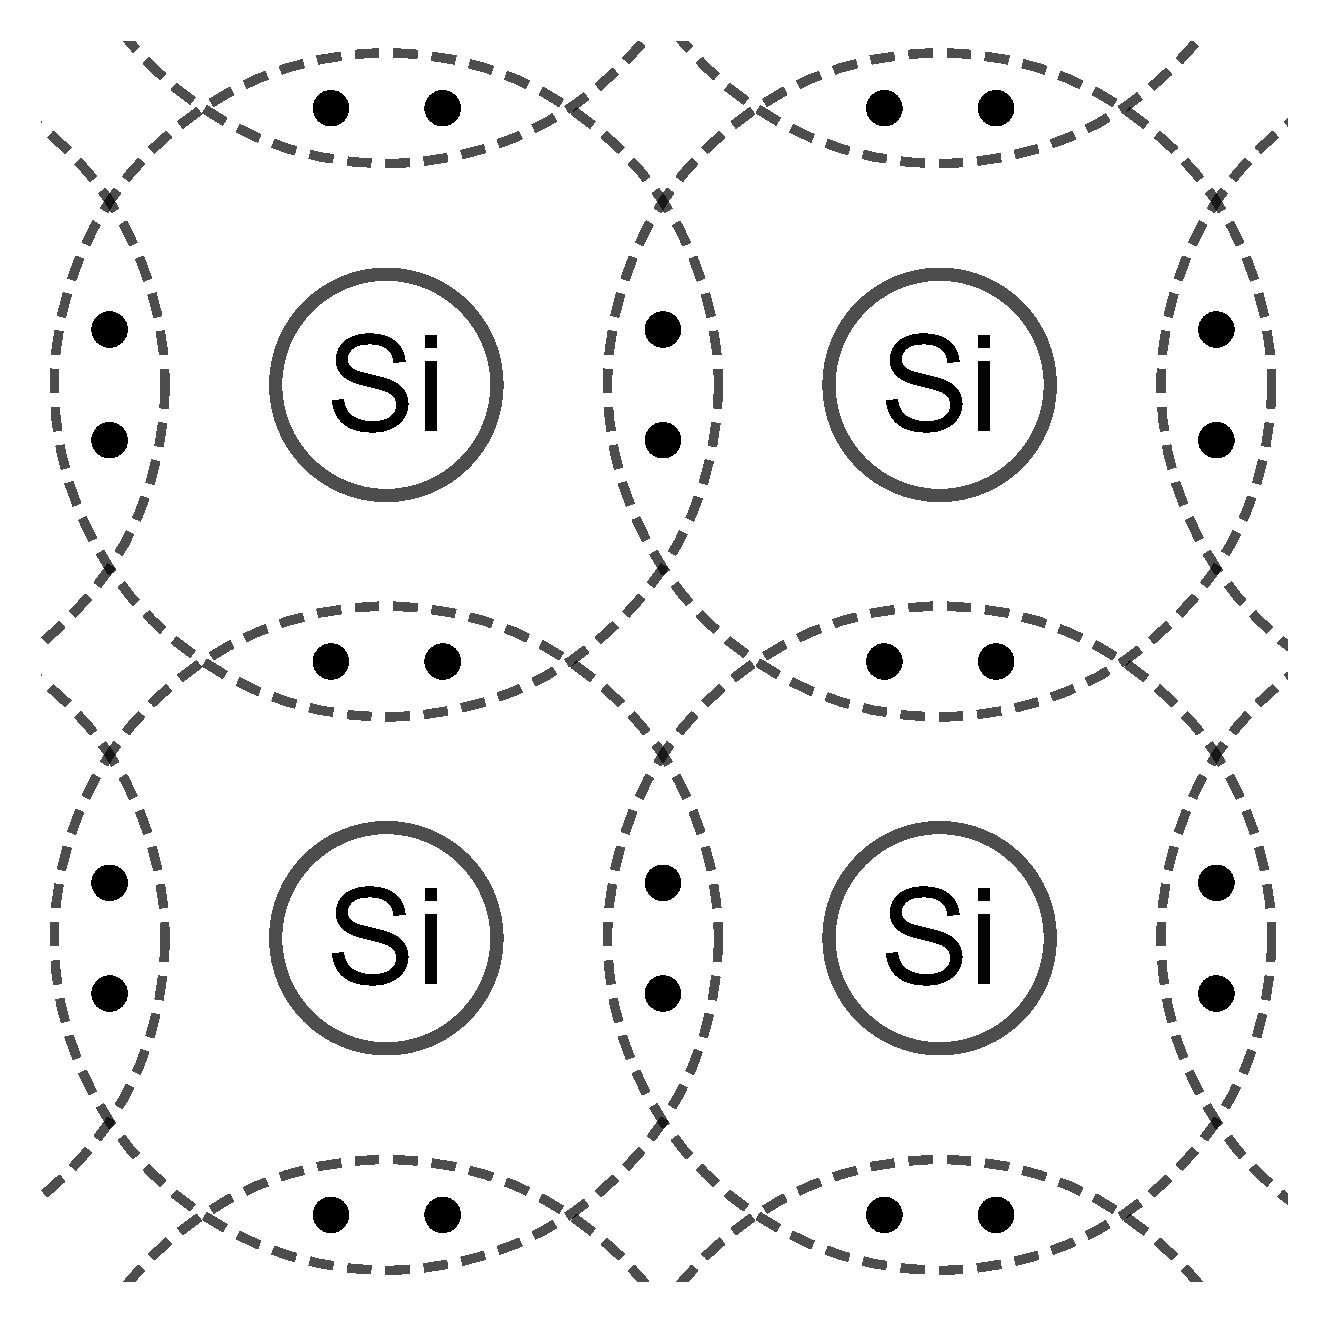
\includegraphics[width=0.35\textwidth]{本征半导体.pdf}
	\caption{本征半导体}
	\label{fig:本征半导体}
\end{figure}
\Par 在外电场的作用下,自由电子做定向移动,形成电子电流.带正电的空穴吸引相邻原子中的价电子来填补,而在该原子的共价键中产生另一个空穴.空穴被填补和相继产生的现象,可以理解为空穴在移动,形成\textbf{空穴电流}.自由电子和空穴都称为\textbf{载流子}.在本征半导体中自由电子和空穴总是成对出现,同时又不断复合.

\subsection{\K PN型半导体}
\Par 由于在本征半导体中自由电子和空穴总是成对出现,这导致每次本征激发产生的载流子很少,为此我们可以提高温度,增加光强,当然,我们最常用的是第三种手段:掺杂其他元素.

\Par 如果我们加入5价原子,比如说磷原子,如图\ref{fig:N型半导体}所示,它就会多出一个电子,掺杂的磷原子越多,自由电子也就越多,这种半导体我们称之为\hl{N型半导体},取Negative之意.在N型半导体中,载流子大多都是电子,但是在本征激发中,也会有少量的空穴载流,因此我们称载流子的多数为\textbf{多子},载流子的少数为\textbf{少子}.在在N型半导体中,多子为电子,少子为空穴.

\begin{figure}[htbp]
    \centering
    \begin{minipage}{0.48\textwidth}
        \centering
	    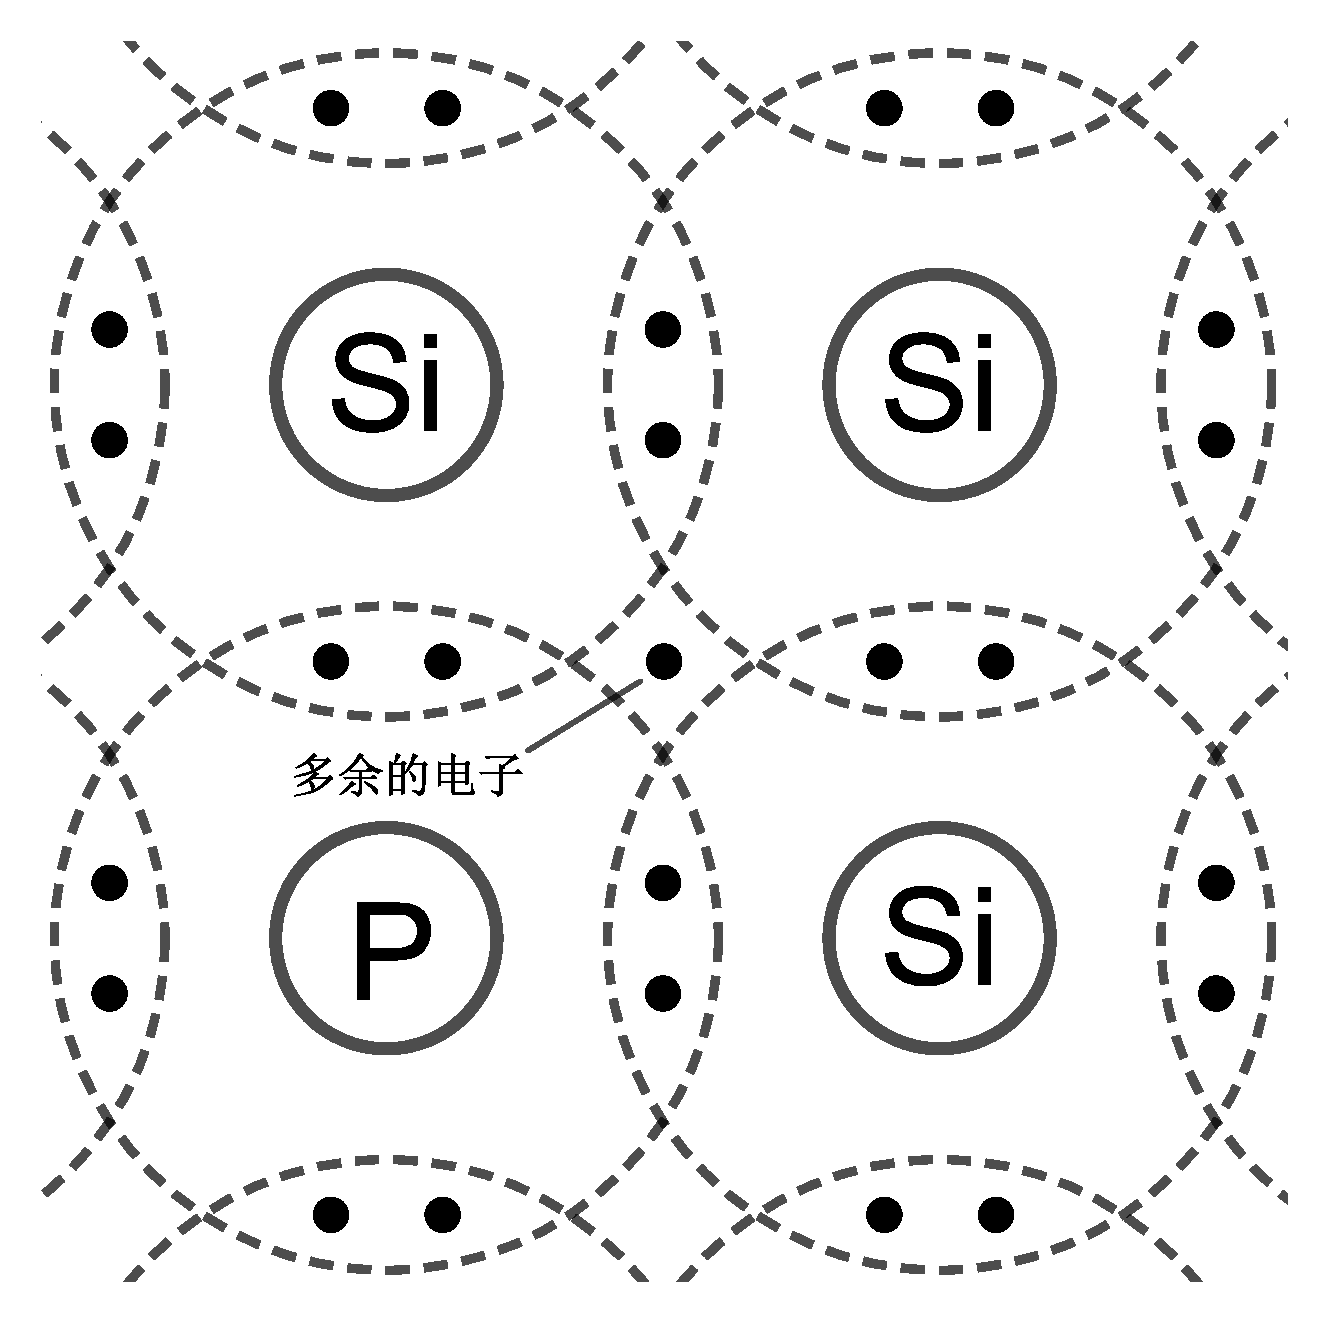
\includegraphics[width=0.65\textwidth]{N型半导体.pdf}
	    \caption{N型半导体}
	    \label{fig:N型半导体}
        \end{minipage}
    \begin{minipage}{0.48\textwidth}
        \centering
	    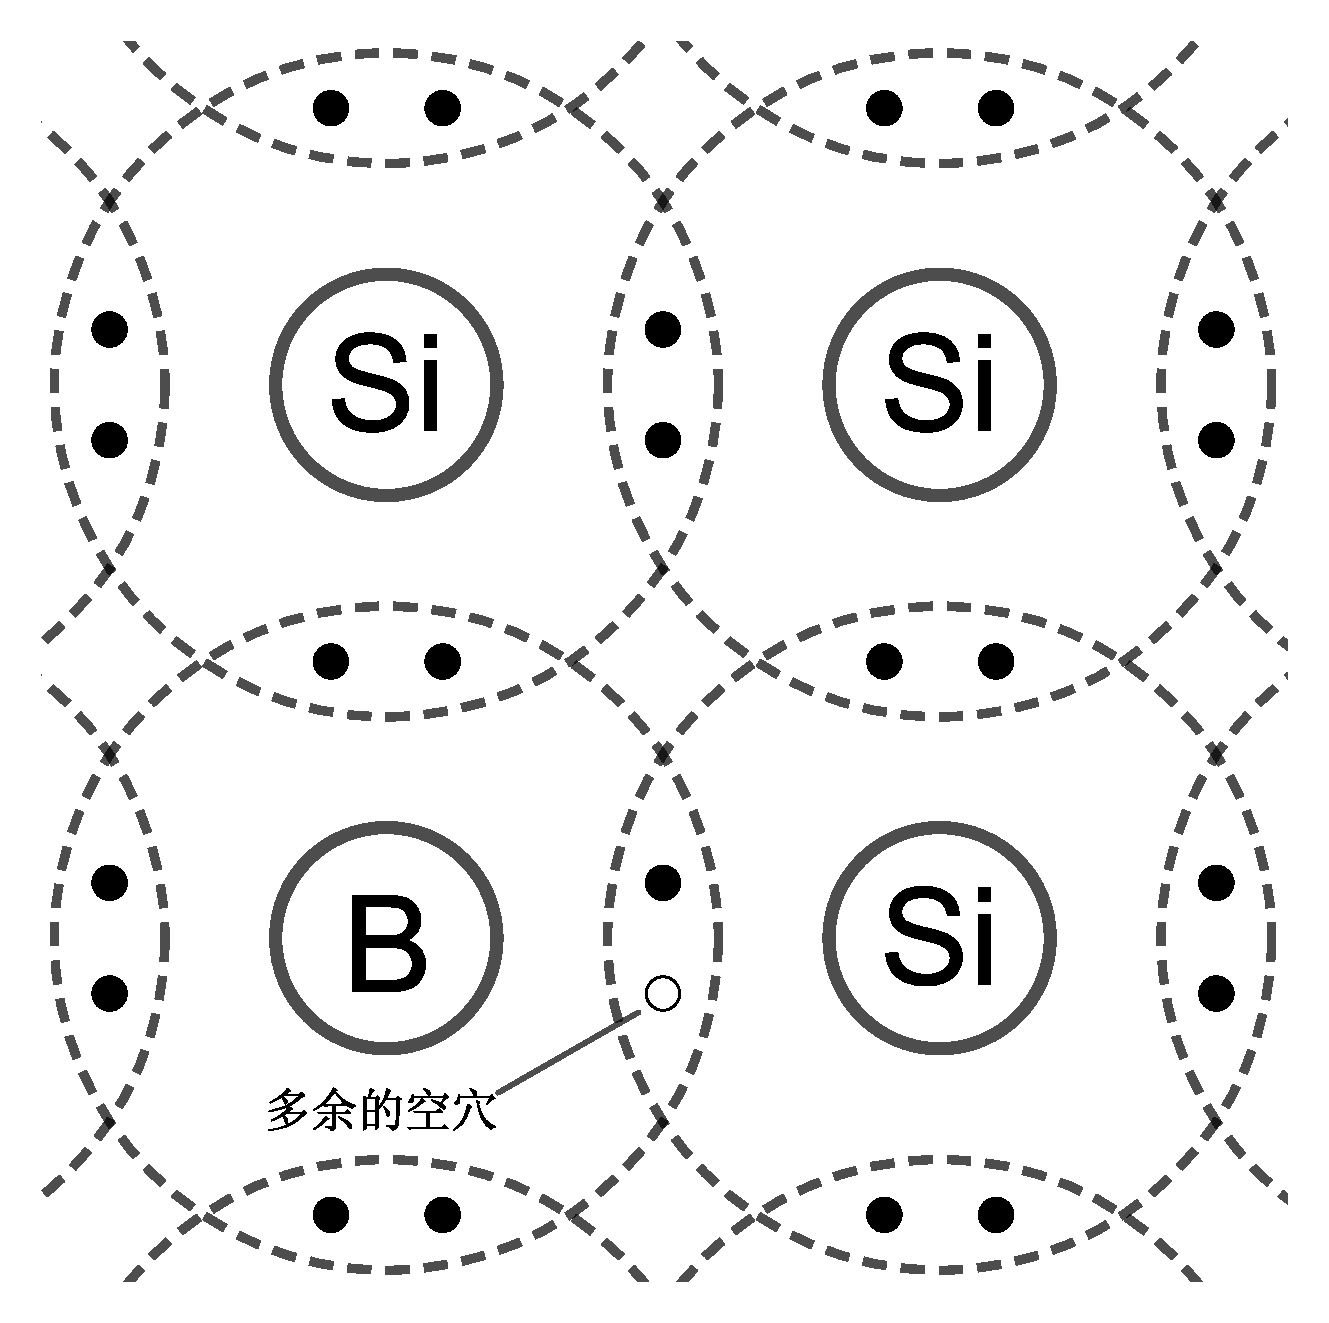
\includegraphics[width=0.65\textwidth]{P型半导体.pdf}
	    \caption{P型半导体}
	    \label{fig:P型半导体}
    \end{minipage}
\end{figure}

\Par 如果我们加入3价原子,比如说硼原子,如图\ref{fig:P型半导体}所示,它就会在共价键中缺少一个电子,从而多出一个空穴,掺杂的硼原子越多,空穴也就越多,这种半导体我们称之为\hl{P型半导体},取Positive之意.在P型半导体中,多子为空穴,少子为电子.

\subsection{\K PN结}

\begin{wrapfigure}{r}{0.35\textwidth}
	\centering
	\includegraphics[width=0.35\textwidth]{PN结.pdf}
	\caption{PN结}
	\label{fig:PN结}
\end{wrapfigure}
\Par 如果我们将一个P型半导体与N型半导体相连,如图\ref{fig:PN结}所示,这个结构被称作\textbf{二极管}.由于P型半导体中的空穴对N型半导体中的电子具有吸引作用,因此N型半导体中的电子会向P型半导体中的空穴移动,并与之复合,而被吸引来却未能完成复合的电子会在两种半导体交界处靠P型半导体侧停留,并在原来N型半导体的位置留下空穴,从而形成了如图\ref{fig:PN结}所示的薄层.这个薄层被称为\hl{PN结},这种现象被称作\textbf{多子的扩散运动}.

\Par PN结形成的内电场会阻止多子的扩散运动,但是少子会被其促进移动,这被称为\textbf{少子的漂移运动}.少子的漂移运动又会削减PN结的厚度,最终与多子的扩散运动形成动态平衡.


\Par 如果我们在PN结两端通电,如图\ref{fig:正向PN结}所示,N型半导体中的电子受外电场的作用与PN结中的空穴结合,从而削弱了PN结的内电场,当外电场强到一定程度时,二极管便被导通了.若是通上反向电压,如图\ref{fig:反向PN结}所示,PN结的内电场会因此变强,从而阻止电流的导通,当然,如果外电压足够大的话,电流还是能导通的,不过这个二极管就坏了.

\begin{figure}[htbp]
	\centering
	\begin{minipage}{0.48\textwidth}
		\centering
		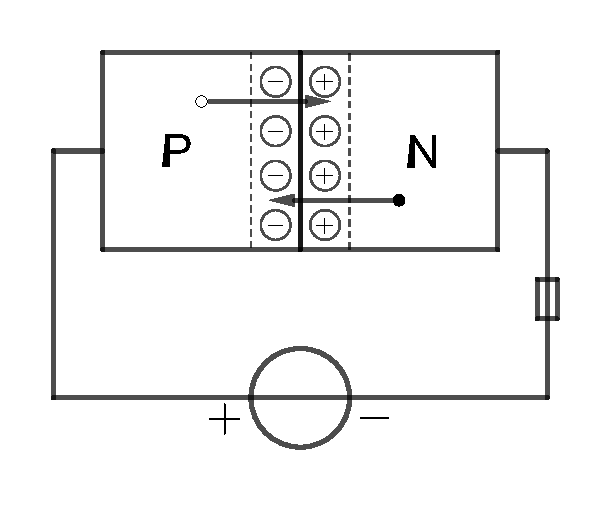
\includegraphics[width=0.85\textwidth]{正向PN结.pdf}
	\caption{正向PN结}
	\label{fig:正向PN结}
	\end{minipage}
	\begin{minipage}{0.48\textwidth}
		\centering
	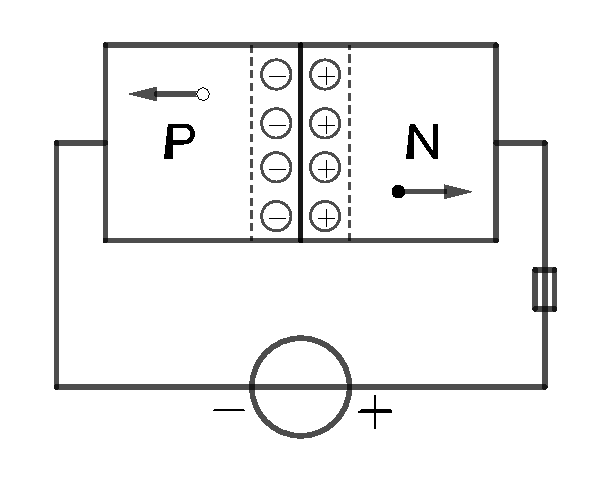
\includegraphics[width=0.85\textwidth]{反向PN结.pdf}
	\caption{反向PN结}
	\label{fig:反向PN结}
	\end{minipage}
\end{figure}
\Par 加上正向电压,往往也需要其高于某个值,电流才能导通,这个值被称作\textbf{死区电压}.一般地,硅管的死区电压约为$0.5\mathrm{V}$,锗管的死区电压约为$0.1\mathrm{V}$,导通后,硅管的电压降约为$0.6\sim 0.7\mathrm{V}$,锗管的电压降约为$0.2\sim 0.3\mathrm{V}$.

\Par 加上反向电压,只要电压够大,电流也能导通,这个电压被称作\textbf{反向击穿电压$U_{BR}$}.

\Par 对于二极管,我们还有以下参数:

\textbf{\circledtext{1}最大整流电流$\boldsymbol{I}_{\mathbf{OM}}$}

最大整流电流是指二极管长时间使用时,允许流过二极管的最大正向平均电流.

\textbf{\circledtext{2}反向工作峰值电压$\boldsymbol{U}_{\mathbf{RWM}}$}

它是保证二极管不被击穿而给出的反向峰值电压,一般是反向击穿电压的1/2或2/3.

\textbf{\circledtext{3}反向峰值电流$\boldsymbol{I}_{\mathbf{RM}}$}

它是指在二极管上加反向工作峰值电压时的反向电流值.

